\documentclass[12pt]{ctexart}
\usepackage{amsmath,graphicx,textcomp,subfigure,indentfirst,ctex,color,float}
\usepackage{xcolor}

\title{Lecture3}
\author{赵思逸}
\date{\today}
\newcommand{\new}[1]{\textcolor{blue}{#1}}

\begin{document}

\maketitle


\section{宇宙学红移(cosmological redshift)}

宇宙学红移:由于宇宙整体膨胀造成的红移。
\par 多普勒红移:在平直时空下由于相对运动速度造成的红移。

\begin{figure}[!hbtp]
    \centering
    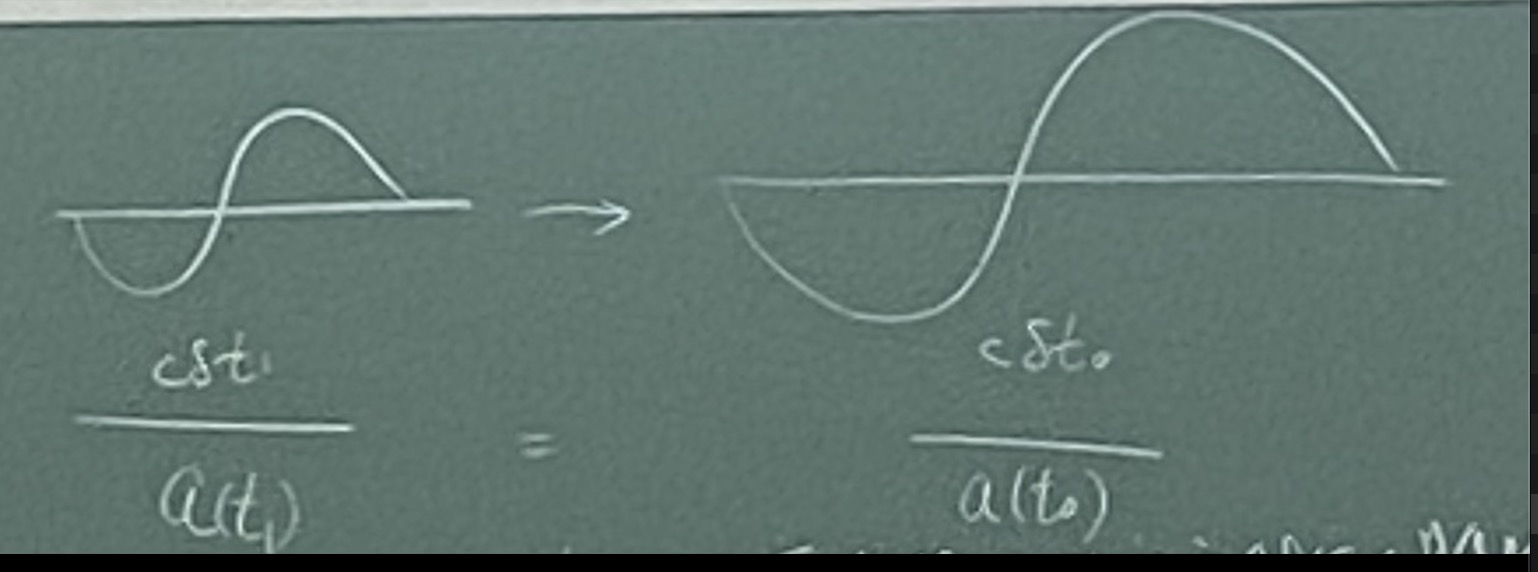
\includegraphics[width=0.8\textwidth]{figures/lambda.jpg}
    \caption{波长随时空膨胀}
\end{figure}
宇宙学红移的推导:光在$t_1$发射,在$t_0$接收,波长随时空膨胀
$\frac{c\delta t_1}{a(t_1)} = \frac{c\delta t_0}{a(t_0)}$,$t_1$时刻$\nu_1 = 1/\delta t_1$,$t_0$时刻$\nu_0 = 1/\delta t_0$,可得 
\begin{equation}
    1+z\equiv \frac{\lambda_\text{obs}}{\lambda_\text{emit}} = \frac{\nu_1}{\nu_0} = \frac{\delta t_0}{\delta t_1}= \frac{a(t_0)}{a(t_1)} >1
\end{equation}

小结:我们定义今天的尺度因子 $a(t_0)\equiv a_0$,则有 
\begin{equation}
    1+z=\frac{a_0}{a(t)}
\end{equation}

我们可以用时间$t$,红移$z$,尺度因子$a$作为“时间变量”来描述宇宙的历史。
\begin{figure}[!hbtp]
    \centering
    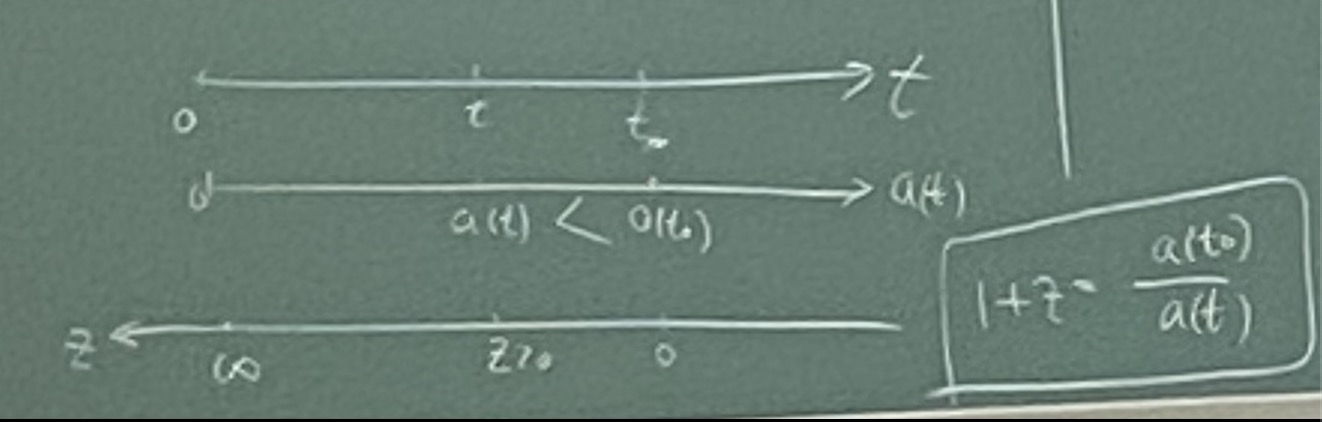
\includegraphics[width=0.8\textwidth]{figures/time.jpg}
    \caption{用时间$t$,红移$z$,尺度因子$a$作为“时间变量”来描述宇宙的历史}
\end{figure}

\section{时空的几何结构}
\subsection{度规}
为了方便推广,我们对平直时空定义 $x^0=ct$, $x^1 = x$, $x^2=y$, $x^3=z$,即$x^\mu=(ct,x,y,z)$,其中$\mu = 0,1,2,3$。
时空间隔(spacetime interval)表示为 $dx^\mu=(cdt,dx,dy,dz)$.

时空线元(spacetimeline element) 是$ds^2=-c^2dt^2 + dx^2 + dy^2 + dz^2=\sum_{\mu,\nu=0}^3 \eta_{\mu \nu}dx^\mu dx^\nu$ ,其中$\eta_{\mu\nu}$叫做度规(metric).

\begin{equation} \label{eq:eta}
    \eta_{\mu\nu} = \left(\begin{array}{llll}-1 & 0 & 0 & 0 \\ 0 & 1 & 0 & 0 \\ 0& 0& 1 &0 \\ 0 & 0&0&1\end{array}\right)
\end{equation}
是平直时空的度规,叫闵可夫斯基度规(Minkowski metric)。

更一般地,$x^\mu$可以是任意坐标系,度规改用  $g_{\mu \nu}$表示,(因为 $\eta_{\mu\nu}$ 一般特指式(\ref{eq:eta}) )
即$ds^2=\sum_{\mu,\nu=0}^3g_{\mu \nu}dx^\mu dx^\nu$ ,其中 $g_{\mu \nu}$可以是坐标的函数。 

提问:度规可以写成坐标的函数,是否一定表示弯曲时空?
\par 答:不是,可能是因为坐标变换。比如平直时空在球坐标下的度规为

$$g_{\mu\nu} = \left(\begin{array}{llll}-1 & 0 & 0 & 0 \\ 0 & 1 & 0 & 0 \\ 0& 0& r^2 &0 \\ 0 & 0&0& r^2 \sin^2 \theta\end{array}\right)$$

那么如何判断是否是平直时空呢?寻找坐标变换下的不变量(比如标量),具体到这个问题,需要计算里奇标量 (Ricci scalar) $R(g_{\mu\nu})$. 平直时空的Ricci scalar为0. 以此可以分辨平直时空与弯曲时空。 

\subsection{共动坐标(comoving frame)下的度规}

取某一时刻$t_\text{com}$的物理距离为坐标距离,定义此时刻尺度因子
\newline $a(t_\text{com})=1$。到$t_1$时刻,宇宙经过膨胀,物理距离=坐标距离$\times a(t_1)$.

共动坐标下三维空间部分的线元$dS_\text{3D}^2 = dx^2+dy^2+dz^2=dr^2+r^2 d\Omega^2$,其中立体角 $d\Omega^2 = d\theta^2 + \sin^2\theta d\phi^2$ 

平直时空下,$ds^2=-c^2dt^2 + dS_\text{3D}^2$。

膨胀宇宙中,$ds^2=-c^2dt^2 + a^2(t) dS_\text{3D}^2$,空间部分可以平直也可以弯曲。

\colorbox{yellow}{我们考虑度规的空间部分。}
因为宇宙学原理,宇宙在空间上是均匀、各向同性的,要求度规的空间部分满足平移和旋转对称性。
符合条件的有且只有三种情况:(证明可参考温伯格的《Gravitation and Cosmology》Sec. 13.2.)
\begin{enumerate}
    \item (最简单的就是)三维平直的欧式空间 $dS_\text{3D}^2 = d\vec{x}^2$,这种情况下,通常可以选择$a(t_\text{today})=1$。
    \item 嵌在四维欧式空间中的三维球面(可用二维球来理解) $dS_\text{3D}^2 = d\vec{x}^2 + dz_4^2$,有球面限制条件$z_4^2 + \vec{x}^2 = R^2$,剩下3个自由度。其中$R$是“球的半径”,是个常数,可以通过对共动坐标的选取使$R=1$,注意这个选取相当于把球半径的物理长度$R=1$的时刻选定为共动坐标的时刻$t_\text{com}$。在这种选择下,在$t$时刻的球半径的物理长度等于$t$时刻的尺度因子$a(t)$,也就是说,此时不能随意选择$a(t_\text{today})=1$,因为$a(t_\text{today})=$今天的球半径的物理长度。
    \item 嵌在四维\underline{赝欧式}空间中的三维\underline{超球面}(可用二维双曲面来理解) \\ $dS_\text{3D}^2 = d\vec{x}^2 - dz_4^2$,有限制条件$z_4^2 - \vec{x}^2 = 1$,剩下3个自由度。已经通过对共动坐标的选取使$R=1$。
\end{enumerate}

综合后两种情况:$dS_\text{3D}^2 = d\vec{x}^2 \pm dz_4^2$,限制条件$z_4^2 \pm \vec{x}^2 = 1$,可得

\begin{equation} \label{eq:dS3D}
    dS_\text{3D}^2 = d\vec{x}^2 \pm \frac{(\vec{x} \cdot d\vec{x})^2}{1\mp \vec{x}^2} = d\vec{x}^2 +  \frac{K(\vec{x} \cdot d\vec{x})^2}{1-K \vec{x}^2}
\end{equation}
其中定义了
\begin{equation}
    K= \begin{cases}+1 & \text { 球面,正曲率,有限体积,无边界} \\ 0 & \text { 欧氏,平直,无限体积,无边界 } \\ -1 & \text { 超球面,负曲率,无限体积,无边界} \end{cases}
\end{equation}
式(\ref{eq:dS3D})第二个等号综合了全部三种情况。

加上时间部分,\colorbox{yellow}{总体的时空度规}是 
\begin{equation}
    ds^2=-c^2dt^2 + a^2(t) \left[d\vec{x}^2 +  \frac{K(\vec{x} \cdot d\vec{x})^2}{1-K \vec{x}^2}\right]
\end{equation}

上式的空间部分$\vec{x}$就是我们日常看到的三维空间,但是在宇宙学中的度规可以不是欧几里德空间的度规(即闵氏度规的空间部分),所以叫“准笛卡尔”坐标(quasi-Cartesian coordinates)。我们将$\vec{x}$转换为球坐标系,可以方便与观测比较。这里球坐标系的定义与平直的欧几里德空间里一样。在球坐标系下,度规写为
\begin{equation}
    ds^2=-c^2dt^2 + a^2(t) \left[ \frac{dr^2}{1-Kr^2} + r^2 d\Omega^2 \right]
\end{equation}

称为 Friedmann-Lemître-Robertson-Walker (FLRW/FRW)度规。

\end{document}
